\documentclass[tikz,border=6pt]{standalone}
\usepackage[T1]{fontenc}
\usepackage[utf8]{inputenc}
\usepackage{pgfplots}
\pgfplotsset{compat=1.18}
\begin{document}
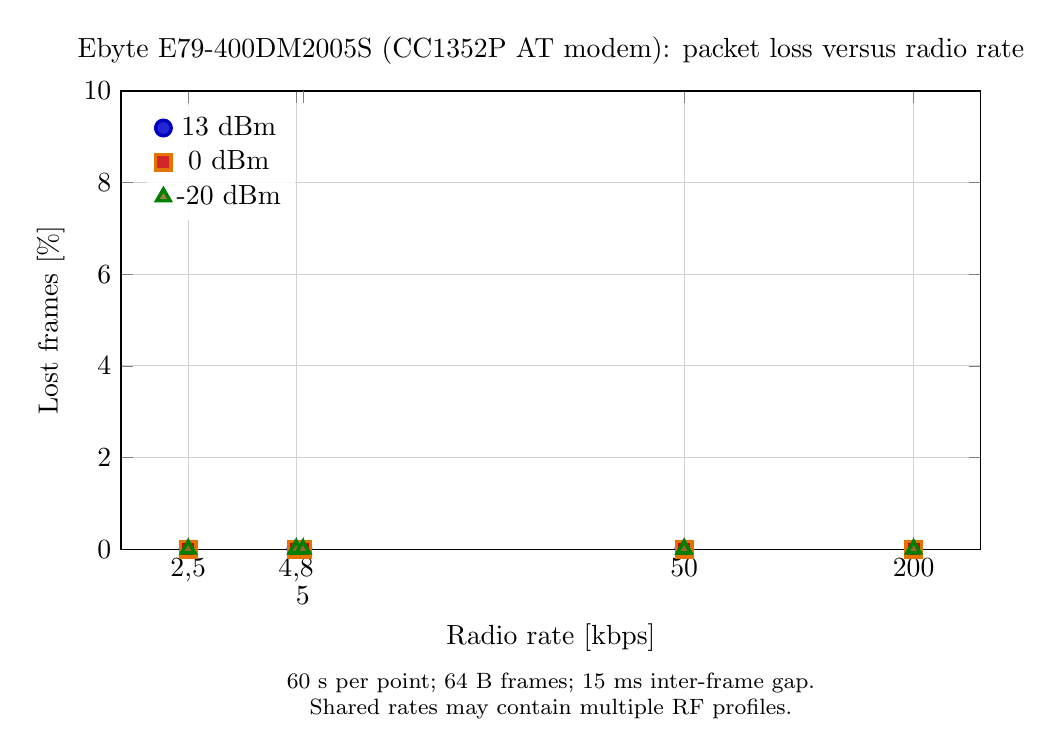
\begin{tikzpicture}
\begin{axis}[width=12.5cm, height=7.4cm,
  title={Ebyte E79-400DM2005S (CC1352P AT modem): packet loss versus radio rate},
  xmode=log, log basis x=10,
  xmin=1.66666667, xmax=300, xtick={2.5,4.8,50,200},
  xticklabels={2{,}5,4{,}8,50,200}, ymin=0, ymax=10,
  extra x ticks={5}, extra x tick labels={5},
  extra x tick style={grid=none, xticklabel style={yshift=-0.35cm}},
  xlabel={Radio rate [kbps]}, ylabel={Lost frames [\%]},
  grid=both, minor grid style={gray!15}, major grid style={gray!35},
  every axis plot/.append style={line width=1.25pt, mark size=2.8pt},
  legend style={draw=none, fill=white, fill opacity=0.85, text opacity=1,
    at={(0.03,0.97)}, anchor=north west, legend columns=1},
]
\addplot+[blue!75!black, only marks, mark=*] coordinates {(2.5,0) (4.8,0) (4.8,0) (5,0) (50,0) (50,0) (200,0)};
\addlegendentry{13 dBm}
\addplot+[orange!90!black, only marks, mark=square*] coordinates {(2.5,0) (4.8,0) (4.8,0) (5,0) (50,0) (50,0) (200,0)};
\addlegendentry{0 dBm}
\addplot+[green!50!black, only marks, mark=triangle*] coordinates {(2.5,0) (4.8,0) (4.8,0) (5,0) (50,0) (50,0) (200,0)};
\addlegendentry{-20 dBm}
\end{axis}
\node[font=\footnotesize, align=center, text width=12cm, anchor=north]
  at ([yshift=-1.45cm]current axis.south)
  {60 s per point; 64 B frames; 15 ms inter-frame gap. Shared rates may contain multiple RF profiles.};
\end{tikzpicture}
\end{document}
